\setlength{\epigraphwidth}{.45\textwidth}
\begin{epigraphs}
\qitem{\textit{We know of an ancient radiation\\
That haunts dismembered constellations,\\
A faintly glimmering radio station.}}%
 {---Frank Sinatra, \textsc{Cake}}
\end{epigraphs}

Over the past two decades cosmology has entered the age of \textit{precision cosmology}\footnote{As advocated by Peebles in \cite{Peebles2002}, the era of precision cosmology is the moment when "\textit{all the important parameters will be established to one significant figure of merit or better, within the cosmological model.}"}: the flood of data collected by  cosmological experiments have transformed cosmology from a data-starving field into a data-driven field, which allows cutting-edge theories to be tested. 
%Nowadays much of the observers and experimentalists efforts are devoted to boost detectors sensitivities as well as to improve analysis techniques in order to shrink the error bars, while theorists struggle to sharpen our understanding of the pressing theoretical issues.
A wide set of cosmological observations \citep{Weinberg2008} have allowed us to summarize our fair understanding of the basic properties of the Universe in the concordance cosmological model - also known as $\Lambda$CDM model - built on the solid theoretical premises of Einstein's General Relativity. Despite the remarkable success in fitting the data, the standard model presents several puzzles on which light needs to be shed. For example, combining different cosmological data sets \citep{PlanckCollaboration2015b}, baryonic matter can account for only 5\% of the mass-energy budget of the Universe, while approximately 25\% is in the form a \textit{dark} component, namely the Dark Matter (DM) whose properties and features are not known yet. Moreover, the mechanism sourcing the late-time accelerated expansion of the Universe, whether being associated to some other dark component dubbed Dark Energy (DE) or to modifications of the underlying theory of gravity (MG), remains elusive.

Most of the information about the cosmological properties and parameters comes from accurate measurements of Cosmic Microwave Background (CMB) anisotropies, which provide us a snapshot of the early Universe. However, a wealth of information about the later evolution of the Universe can be gained by studying the interaction between CMB photons and its Large Scale Structure (LSS), giving rise to the so-called CMB \textit{secondary anisotropies}. In this framework, two effects have recently emerged as new promising and powerful tools, the \textit{weak gravitational lensing} of CMB photons and the \textit{kinetic Sunyeav-Zel'dovich effect}. 

CMB lensing is the deflection of photons trajectories due to the intervening matter distribution between the last scattering surface (the edge of the observable Universe) and us. On one hand it encodes a wealth of information about the geometry and the growth of structure in the Universe, on the other it represents a nuisance since it obscures the primordial inflationary polarization $B$-mode signal. In a period of less than 10 years, from 2007 - the year that I enrolled at the university - up to now, CMB lensing science has turned from the detection regime to being a standard cosmological probe. In fact, it is one of the main driver of the upcoming experimental efforts represented by a plethora of ground-based high-sensitivity CMB experiments such as the Simons Array, the South Pole Telescope (SPT-3G), the Advanced Atacama Cosmology Telescope (AdvACT), the Simons Observatory, and CMB-S4 devoted to an exquisite mapping of the CMB lensing sky.

The kinetic Sunyeav-Zel'dovich (kSZ) effect arises from the inverse Compton scattering of CMB photons off of free electrons, and it is specifically sourced by the bulk motion of these electrons with respect to the CMB rest frame. The large-scale momentum field is a powerful cosmological probe that can place tight constraints on the growth of structure and the epoch of reionization in a complementary way with respect to density fluctuations measurements. 

This thesis focuses on how to exploit these two effects to address both cosmological and astrophysical questions, and it features theoretical work, observations, and data analysis. Specifically, we will exploit the synergy between the \textit{Planck} and \textit{Herschel} satellites by developing, validating, and applying cross-correlation algorithms to reconstruct the tomographic signal between the CMB lensing and the positions of the sub-millimeter selected galaxies. As pictorially shown in Fig.~\ref{fig:xc}, such a signal is detectable because we are basically probing the same underlying field, i.e. the integrated matter distribution on cosmological scales.\footnote{As a little disclaimer we note that the (gradients of) gravitational potentials are technically responsible for the deflection of CMB photons rather than the matter distribution itself, though in the standard scenario (General Relativity) the two can be related through the Poisson equation.} Galaxies represent the biased signpost of the DM halos, the most massive of which act as lenses for the CMB photons, providing a clean and independent measure of the relation between luminous and dark matter. Cross-correlation measurements are generically less sensitive to any known (and unknown) systematics, as well as to extract signals hidden in noisy data, even though the full potential of these measurements is still under scrutiny, and it is one of the drivers of the present work. We anticipate that the key aspect of the present work is an accurate interplay between CMB lensing datasets as seen from \textit{Planck} on one side, and an accurate selection of DM tracers on Herschel data on the other. This results in the most accurate detection of the cross-correlation to date, which allows to exploit it to set cosmological constraints from cross-correlations, which will become tighter and tighter in the incoming years. 

The second main topic discussed in this thesis is the impact of modified gravity theories on the kSZ effect of the CMB. Several approaches to detect and study the kSZ have emerged on the market, here we focus on the kSZ signal showing up at small scales in the temperature CMB power spectrum (assuming an efficient foreground removal by means of multi-frequency observations). By being dependent on the details of the growth history, especially at late times, and on the epoch of reionization, the kSZ can be exploited to test gravity on cosmological scales. This field of research is at the early stages of development, though it is very promising both as a cosmological and astrophysical tool. 

\begin{figure} %1
\centering % \begin{center}/\end{center} takes some additional vertical space
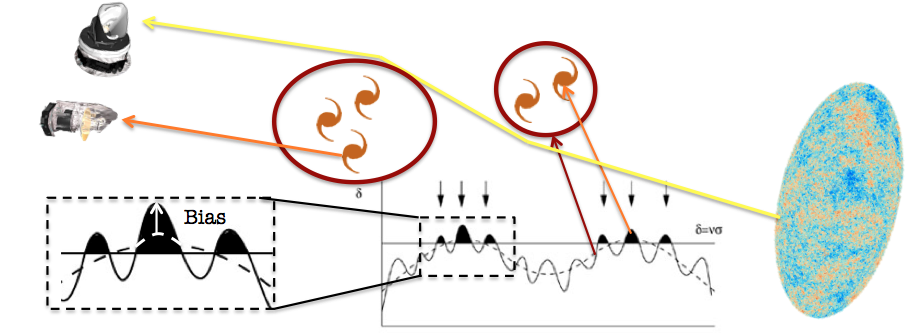
\includegraphics[width=\textwidth]{Introduction/Images/xc}
\caption{Pictorial explanation of the origin of the CMB lensing - galaxy density cross-correlation signal. While CMB photons collected by the \textit{Planck} satellite experience several deflections during their cosmic journey because of the matter perturbations (represented by DM halos), the dusty enshrouded galaxies that reside in these halos emit infrared photons captured by \textit{Herschel}.\label{fig:xc}}
\end{figure}

\myparagraph{Outline of the Thesis}
This thesis is organized as follows. The first two chapters are propaedeutic to follow the main content. In Ch.~\ref{ch:cosmo} we review the basics of the current cosmological model, carefully focusing on the physics and applications of two of the main pillars, the CMB and the weak gravitational lensing. The following chapter, Ch.~\ref{ch:statsdata}, deals with the statistics of random fields, since these are fundamental to model and analyze the data, and provides a thorough description of the exploited \textit{Planck} and \textit{Herschel} datasets. The remaining four chapters represent the core of the work carried out during my Ph.D. and exposed in this thesis. In Ch.~\ref{ch:xc1} we present the first cross-correlation measurement between the \textit{Planck} CMB lensing and the spatial distribution of the high-$z$ ($z \gtrsim 1.5 $) dusty star-forming galaxies detected by \textit{Herschel}-ATLAS, measuring the linear galaxy bias $b$ and reporting a cross-correlation signal somewhat stronger than expected. We improve this analysis with updated datasets in Ch.~\ref{ch:xc2}, where we attempt a first tomographic approach by splitting the galaxy sample in two redshift bins and studying the evolution of the cross-correlation amplitude and galaxy bias over cosmic time. Ch.~\ref{ch:cmbneed} is devoted to the methodology and algorithms to investigate the cross-correlation between CMB and LSS datasets: we discuss the spectral estimation problem in the needlet framework, developing a \texttt{MASTER}-like technique to address the bias induced by heavy masking, and compare it with its harmonic counterpart. In Ch.~\ref{ch:ksz} we consider the capability of the kSZ power spectrum measured by the small-scale CMB telescope to constrain models of modified gravity, in particular we focus on a specific $f(R)$ model, the Hu \& Sawicki one. Finally, we summarize the main results and future perspectives in the Conclusions.






